\documentclass{standalone}
\usepackage[dvipsnames]{xcolor}
\usepackage{tikz}
\usetikzlibrary{shapes}

\begin{document}
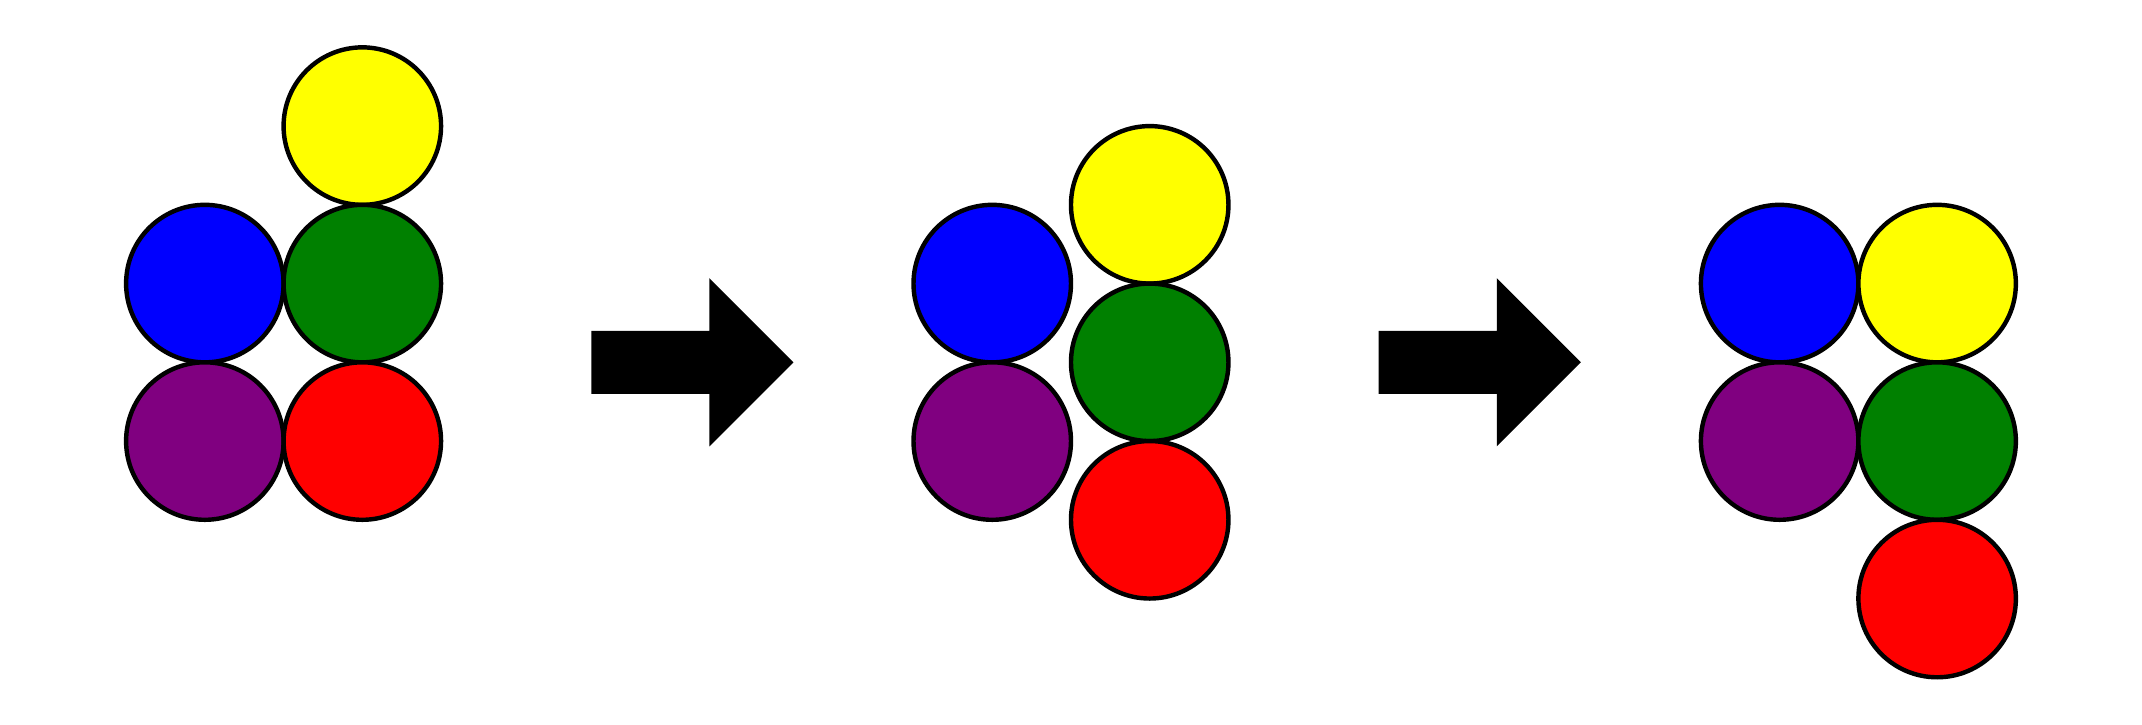
\begin{tikzpicture}[x=1cm, y=1cm]
\node[draw, circle, ultra thick, inner sep=0pt, minimum size=2cm, fill=Yellow] () at (3,2) {};
\node[draw, circle, ultra thick, inner sep=0pt, minimum size=2cm, fill=Blue] () at (1,0) {};
\node[draw, circle, ultra thick, inner sep=0pt, minimum size=2cm, fill=Green] () at (3,0) {};
\node[draw, circle, ultra thick, inner sep=0pt, minimum size=2cm, fill=Purple] () at (1,-2) {};
\node[draw, circle, ultra thick, inner sep=0pt, minimum size=2cm, fill=Red] () at (3,-2) {};

%\node[draw, single arrow, ultra thick, fill=black, inner sep=0pt, minimum height=2.5cm, minimum width=2cm] () at (7,-1) {\phantom{M}};
\node[draw, single arrow, ultra thick, fill=black, inner sep=0pt, minimum height=2.5cm, minimum width=2cm] () at (7,-1) {\phantom{M}};

\node[draw, circle, ultra thick, inner sep=0pt, minimum size=2cm, fill=Yellow] () at (13,1) {};
\node[draw, circle, ultra thick, inner sep=0pt, minimum size=2cm, fill=Blue] () at (11,0) {};
\node[draw, circle, ultra thick, inner sep=0pt, minimum size=2cm, fill=Green] () at (13,-1) {};
\node[draw, circle, ultra thick, inner sep=0pt, minimum size=2cm, fill=Purple] () at (11,-2) {};
\node[draw, circle, ultra thick, inner sep=0pt, minimum size=2cm, fill=Red] () at (13,-3) {};

%\node[draw, single arrow, ultra thick, fill=black, inner sep=0pt, minimum height=2.5cm, minimum width=2cm] () at (15,-1) {\phantom{M}};
\node[draw, single arrow, ultra thick, fill=black, inner sep=0pt, minimum height=2.5cm, minimum width=2cm] () at (17,-1) {\phantom{M}};

\node[draw, circle, ultra thick, inner sep=0pt, minimum size=2cm, fill=Blue] () at (21,0) {};
\node[draw, circle, ultra thick, inner sep=0pt, minimum size=2cm, fill=Yellow] () at (23,0) {};
\node[draw, circle, ultra thick, inner sep=0pt, minimum size=2cm, fill=Purple] () at (21,-2) {};
\node[draw, circle, ultra thick, inner sep=0pt, minimum size=2cm, fill=Green] () at (23,-2) {};
\node[draw, circle, ultra thick, inner sep=0pt, minimum size=2cm, fill=Red] () at (23,-4) {};

%\path (-1.5, -5.25) to (23.5,3.25);
\path (-1.25, -5.25) to (25.25,3.25);

\end{tikzpicture}
\end{document}